\chapter{Testing and Quality Assurance}\label{ch:test}

Testing followed the plan in \Cref{sec:testplan}. The evidence in this chapter comes from two sources:
(1) the automated backend test suite \texttt{app/tests}, run on 16 November 2026 at commit \texttt{60d40f9} on
a Windows~11 laptop with Python~3.13, with all provider keys removed from the environment so that no real AI
service was called; and (2) manual and user tests on the running application with documents the team had
already uploaded. Where a result has not yet been
measured, the table says so instead of giving a number.

\section{Requirements/Specifications-Based System Level Test (Detailed with Test Results)}

\Cref{tab:reqlist} lists the functional requirements, derived from the use cases in \Cref{ch:req}. The
security (SEC-) and AI (R-AI-) requirements are those of \Cref{sec:security,sec:ai-req}.

\begin{table}[!htbp]
\centering
\caption{Functional requirements used for system-level testing}\label{tab:reqlist}
\small
\begin{tabularx}{\textwidth}{@{}l X l l@{}}
\toprule
\textbf{ID} & \textbf{Requirement statement} & \textbf{Must/Want} & \textbf{Use case}\\
\midrule
FR-01 & A user can sign up, log in and log out; protected routes reject requests without a valid token & Must & UC-01\\
FR-02 & A user can upload a PDF, Markdown or text file; invalid, empty, oversized or corrupt files are rejected & Must & UC-02\\
FR-03 & An uploaded document is processed into chunks and its job status is reported & Must & UC-02\\
FR-04 & A user can read a document and annotate it & Must & UC-03\\
FR-05 & A user can generate a Cornell note for a topic & Must & UC-04\\
FR-06 & A user can take a Socratic drill and receive a score, gaps and suggested cards & Must & UC-05\\
FR-07 & Due items are reviewed in sessions and rescheduled with FSRS & Must & UC-06\\
FR-08 & Knowledge Hub answers are grounded in the user's documents with valid citations & Must & UC-07\\
FR-09 & A user can generate a quiz, attempt it and get a server-side score & Must & UC-08\\
FR-10 & A user can see learning progress computed from recorded activity & Want & UC-09\\
FR-11 & A user can save, test and delete personal provider keys; keys are never shown in full & Must & UC-10\\
FR-12 & A user can view, edit and reset system prompts & Want & UC-11\\
FR-13 & A user can generate, edit and delete flashcard sets grounded in a document & Must & UC-12\\
FR-14 & One user can never read or change another user's data & Must & all\\
\bottomrule
\end{tabularx}
\end{table}

The system-level test cases are grouped by module in \Cref{tab:tc_auth,tab:tc_docs,tab:tc_review,tab:tc_hub,tab:tc_gen,tab:tc_byok,tab:tc_manual}.
Each automated case names the pytest test that implements it; the \emph{Actual} column is the observed
result of the run described above. The results of every automated test file are in
Appendix~B (\Cref{tab:fulltc}).

\newcommand{\tchead}[2]{%
\small
\begin{tabularx}{\textwidth}{@{}l X l X@{}}
\toprule
\textbf{Project Name} & RecaLL & \textbf{Module Name} & #1\\
\textbf{Created By} & #2 & \textbf{Reviewed By} & Al Rubayet\\
\textbf{Date of Creation} & 16-11-2026 & \textbf{Date of Review} & 18-11-2026\\
\bottomrule
\end{tabularx}\par\vspace{4pt}}
\newcommand{\tcbody}{\setlength{\tabcolsep}{3pt}\footnotesize}
\newcolumntype{Y}{>{\raggedright\arraybackslash}X}

\begin{table}[!htbp]
\centering
\caption{System-level test cases -- module: authentication and accounts}\label{tab:tc_auth}
\tchead{Authentication}{Md.\ Rony Hossain}
\tcbody
\begin{tabularx}{\textwidth}{@{}l Y Y Y l@{}}
\toprule
\textbf{TC ID} & \textbf{Scenario} & \textbf{Expected} & \textbf{Actual (test)} & \textbf{Status}\\
\midrule
TC-AU-01 & Sign up with valid data & Account and workspace created, token returned & As expected (\texttt{test\_signup\_flow}) & Passed\\
TC-AU-02 & Sign up with an e-mail already used & HTTP 409, no second account & As expected (\texttt{test\_duplicate\_signup\_conflict}) & Passed\\
TC-AU-03 & Log in with correct password & JWT returned & As expected (\texttt{test\_login\_flow}) & Passed\\
TC-AU-04 & Call \texttt{/auth/me} with and without token & 200 with token, 401 without & As expected (\texttt{test\_get\_me\_with\_and\_without\_token}) & Passed\\
TC-AU-05 & Invalid e-mail format / short password / missing fields & Rejected with a validation error & As expected (\texttt{test\_validation}, 3 tests) & Passed\\
TC-AU-06 & Repeated password-change attempts & Throttled with HTTP 429 & As expected (\texttt{test\_password\_change\_rate\_limiting}) & Passed\\
TC-AU-07 & Expired or tampered JWT & Rejected & As expected (\texttt{test\_jwt\_token\_expiration}, \texttt{test\_jwt\_tampered\_token\_rejected}) & Passed\\
\bottomrule
\end{tabularx}
\end{table}

\begin{table}[!htbp]
\centering
\caption{System-level test cases -- module: document upload and processing}\label{tab:tc_docs}
\tchead{Documents}{Md.\ Rony Hossain}
\tcbody
\begin{tabularx}{\textwidth}{@{}l Y Y Y l@{}}
\toprule
\textbf{TC ID} & \textbf{Scenario} & \textbf{Expected} & \textbf{Actual (test)} & \textbf{Status}\\
\midrule
TC-DOC-01 & Upload a valid PDF & Job completes; document ready with chunks & As expected (\texttt{test\_pdf\_upload\_and\_pipeline\_success}) & Passed\\
TC-DOC-02 & Upload Markdown / text & Processed like a PDF & As expected (2 tests) & Passed\\
TC-DOC-03 & Upload an empty file & Rejected & As expected (\texttt{test\_empty\_file\_rejected}) & Passed\\
TC-DOC-04 & Upload a file whose bytes are not a PDF & Rejected by magic-byte check & As expected (\texttt{test\_corrupt\_pdf\_rejected\_by\_magic\_bytes}) & Passed\\
TC-DOC-05 & Unsupported extension / oversized file & Rejected with an error & As expected (2 tests) & Passed\\
TC-DOC-06 & Re-process the same document & No duplicate chunks & As expected (\texttt{test\_pipeline\_idempotency}) & Passed\\
TC-DOC-07 & Delete a document & Chunks and jobs deleted with it & As expected (\texttt{test\_cascade\_deletion}) & Passed\\
\bottomrule
\end{tabularx}
\end{table}

\begin{table}[!htbp]
\centering
\caption{System-level test cases -- module: review and FSRS scheduling}\label{tab:tc_review}
\tchead{Reviews (FSRS)}{Md.\ Rony Hossain}
\tcbody
\begin{tabularx}{\textwidth}{@{}l Y Y Y l@{}}
\toprule
\textbf{TC ID} & \textbf{Scenario} & \textbf{Expected} & \textbf{Actual (test)} & \textbf{Status}\\
\midrule
TC-RV-01 & Rate items Again/Hard/Good/Easy & FSRS state and due date change correctly & As expected (\texttt{test\_fsrs\_state\_transitions\_and\_ratings}) & Passed\\
TC-RV-02 & Same rating at a fixed time & Same schedule (deterministic) & As expected (\texttt{test\_fsrs\_deterministic\_fixed\_timestamp}) & Passed\\
TC-RV-03 & Send an invalid rating & Rejected with a validation error & As expected (\texttt{test\_invalid\_rating\_rejected}) & Passed\\
TC-RV-04 & Open the queue & Overdue first, then due now & As expected (\texttt{test\_review\_queue\_ordering\_and\_filtering}) & Passed\\
TC-RV-05 & Request the next card & Answer hidden until revealed & As expected (\texttt{test\_review\_session\_lifecycle\_and\_masking}) & Passed\\
TC-RV-06 & Rate the same item twice & Second rating refused (409) & As expected (\texttt{test\_prevent\_double\_rating\_idempotency}) & Passed\\
TC-RV-07 & Abandon a session & Completed reviews are kept & As expected (\texttt{test\_session\_abandonment\_preserves\_completed\_reviews}) & Passed\\
TC-RV-08 & Review uses no AI credit & Credit balance unchanged & As expected (\texttt{test\_zero\_ai\_credits\_used\_for\_reviews}) & Passed\\
\bottomrule
\end{tabularx}
\end{table}

\begin{table}[!htbp]
\centering
\caption{System-level test cases -- module: Knowledge Hub (retrieval and chat)}\label{tab:tc_hub}
\tchead{Knowledge Hub}{Md.\ Rony Hossain}
\tcbody
\begin{tabularx}{\textwidth}{@{}l Y Y Y l@{}}
\toprule
\textbf{TC ID} & \textbf{Scenario} & \textbf{Expected} & \textbf{Actual (test)} & \textbf{Status}\\
\midrule
TC-KH-01 & Ask a question answered in one chunk & Answer cites that chunk & As expected (\texttt{test\_case\_a\_direct\_retrieval}) & Passed\\
TC-KH-02 & Answer needs several chunks & All needed chunks retrieved & As expected (\texttt{test\_case\_c\_multi\_chunk\_answer}) & Passed\\
TC-KH-03 & Ask about something not in the documents & Says the material does not contain it & As expected (\texttt{test\_case\_d\_missing\_knowledge\_behavior}) & Passed\\
TC-KH-04 & Restrict the question to one document & Only that document is searched & As expected (\texttt{test\_case\_f\_document\_scope}) & Passed\\
TC-KH-05 & Model cites a source that was not retrieved & Citation removed & As expected (\texttt{test\_citation\_validator\_case\_insensitivity\_and\_spacing}) & Passed\\
TC-KH-06 & Document text tries to close the reference tag & Delimiters neutralised & As expected (\texttt{test\_prompt\_injection\_delimiter\_sanitization}) & Passed\\
TC-KH-07 & Streamed answer & Server-sent events in order & As expected (\texttt{test\_rag\_streaming\_sse}) & Passed\\
\bottomrule
\end{tabularx}
\end{table}

\begin{table}[!htbp]
\centering
\caption{System-level test cases -- module: flashcard and quiz generation}\label{tab:tc_gen}
\tchead{Flashcards and quizzes}{Md.\ Rony Hossain}
\tcbody
\begin{tabularx}{\textwidth}{@{}l Y Y Y l@{}}
\toprule
\textbf{TC ID} & \textbf{Scenario} & \textbf{Expected} & \textbf{Actual (test)} & \textbf{Status}\\
\midrule
TC-GEN-01 & Generate cards / quiz without login & HTTP 401 & As expected (2 tests) & Passed\\
TC-GEN-02 & Generate from another user's document & Refused & As expected (2 tests) & Passed\\
TC-GEN-03 & Generated items cite their sources & Citations valid; invented ones stripped & As expected (4 tests) & Passed\\
TC-GEN-04 & Duplicate cards or questions & Removed & As expected (2 tests) & Passed\\
TC-GEN-05 & Document with too little text & Clear ``insufficient material'' error & As expected (2 tests) & Passed\\
TC-GEN-06 & Quiz options invalid (e.g.\ answer not among options) & Rejected by guardrails & As expected (\texttt{test\_option\_validation\_and\_guardrails}) & Passed\\
TC-GEN-07 & Submit an attempt with mixed and blank answers & Deterministic server-side score & As expected (\texttt{test\_deterministic\_scoring\_mixed\_and\_unanswered}) & Passed\\
TC-GEN-08 & Model reply wrapped in Markdown fences & Parsed correctly & As expected (2 tests) & Passed\\
\bottomrule
\end{tabularx}
\end{table}

\begin{table}[!htbp]
\centering
\caption{System-level test cases -- module: provider keys (BYOK) and security primitives}\label{tab:tc_byok}
\tchead{BYOK and security}{Md.\ Rony Hossain}
\tcbody
\begin{tabularx}{\textwidth}{@{}l Y Y Y l@{}}
\toprule
\textbf{TC ID} & \textbf{Scenario} & \textbf{Expected} & \textbf{Actual (test)} & \textbf{Status}\\
\midrule
TC-BY-01 & Save, list and delete a key & Only a masked hint is listed & As expected (\texttt{test\_byok\_crud\_flow}) & Passed\\
TC-BY-02 & Save a key for an unknown provider & Rejected & As expected (\texttt{test\_byok\_invalid\_provider}) & Passed\\
TC-BY-03 & Encrypt then decrypt a key; alter the ciphertext & Round trip works; tampering detected & As expected (2 tests) & Passed\\
TC-BY-04 & Responses of generation endpoints & No secret appears in any response & As expected (\texttt{test\_zero\_secret\_leak}, 2 tests) & Passed\\
TC-BY-05 & Two hashes of the same password & Different salts; verification works & As expected (2 tests) & Passed\\
TC-BY-06 & File name with \texttt{../} path traversal & Refused & As expected (\texttt{test\_storage\_path\_traversal\_prevention}) & Passed\\
TC-BY-07 & Production start with default secrets & Start-up refused & As expected (2 tests) & Passed\\
\bottomrule
\end{tabularx}
\end{table}

The study features that run on the older routes (reader and annotations, Cornell notes, Socratic drill and
prompt editing) have no automated tests in \texttt{app/tests}. They were tested manually on the running
application with documents already uploaded by the team, as listed in \Cref{tab:tc_manual}.

\begin{table}[!htbp]
\centering
\caption{System-level test cases -- manual tests of the study features}\label{tab:tc_manual}
\tchead{Study features (manual)}{Md.\ Rony Hossain}
\tcbody
\begin{tabularx}{\textwidth}{@{}l Y Y Y l@{}}
\toprule
\textbf{TC ID} & \textbf{Scenario} & \textbf{Expected} & \textbf{Actual} & \textbf{Status}\\
\midrule
TC-MAN-01 & Open an uploaded lecture PDF in the reader and select a topic & PDF page and topic tree shown side by side & Shown (\Cref{fig:ss-reader}) & Passed\\
TC-MAN-02 & Generate a Cornell note for one topic & Structured note with cue questions & Generated (\Cref{fig:ss-cornell}) & Passed\\
TC-MAN-03 & Start a Socratic drill on a topic & Two reasoning questions with a hint & Generated (\Cref{fig:ss-drill}) & Passed\\
TC-MAN-04 & Submit a drill answer & Score, gaps and suggested cards & Strong answers scored 95 and 100 (mastered); weak answers 0 (misconception) with 2 cards & Passed\\
TC-MAN-05 & Ask the Knowledge Hub about an uploaded chapter & Answer with [S$n$] marker & Answered with [S1] (\Cref{fig:ss-hub}) & Passed\\
TC-MAN-06 & Edit a system prompt, then reset it & Override used, then default restored & Override saved and shown as customised; an override with an unknown variable was refused (400); reset restored the default & Passed\\
TC-MAN-07 & Highlight text and ask for an explanation & Explanation saved as annotation & Explanation of a passage on page 25 of the AI lecture saved as an annotation & Passed\\
\bottomrule
\end{tabularx}
\end{table}

\section{Traceability of Test Cases to Use Cases}

\Cref{tab:trace} maps every test group to the requirements and use cases it covers. Every Must requirement
has at least one test. FR-04, FR-05, FR-06 and FR-12 are covered by the manual tests in \Cref{tab:tc_manual}.

\begin{table}[!htbp]
\centering
\caption{Traceability of test cases to requirements and use cases}\label{tab:trace}
\small\setlength{\tabcolsep}{4pt}
\begin{tabularx}{\textwidth}{@{}l X X l@{}}
\toprule
\textbf{Test cases} & \textbf{Requirements} & \textbf{Use cases} & \textbf{Kind}\\
\midrule
TC-AU-01 -- 07 & FR-01, SEC-A1, SEC-A3, SEC-P2 & UC-01 & Automated\\
TC-DOC-01 -- 07 & FR-02, FR-03, SEC-I2 & UC-02 & Automated\\
TC-MAN-01, 07 & FR-04 & UC-03 & Manual\\
TC-MAN-02 & FR-05 & UC-04 & Manual\\
TC-MAN-03, 04 & FR-06, R-AI-03, R-AI-04 & UC-05 & Manual\\
TC-RV-01 -- 08 & FR-07, R-AI-02 & UC-06 & Automated\\
TC-KH-01 -- 07, TC-MAN-05 & FR-08, R-AI-05, R-AI-06, R-AI-07 & UC-07 & Both\\
TC-GEN-01 -- 08 & FR-09, FR-13, R-AI-10, SEC-I4 & UC-08, UC-12 & Automated\\
\texttt{test\_analytics} (12 tests) & FR-10 & UC-09 & Automated\\
TC-BY-01 -- 07 & FR-11, SEC-P3, SEC-I6 & UC-10 & Automated\\
TC-MAN-06 & FR-12, R-AI-13 & UC-11 & Manual\\
\texttt{test\_user\_isolation\_matrix} (26 tests) & FR-14, SEC-A2 & all & Automated\\
\bottomrule
\end{tabularx}
\end{table}

\section{Techniques Used for Test Generation}

\begin{itemize}
  \item \textbf{Equivalence partitioning.} Upload inputs were split into valid PDF, Markdown and text files and
  invalid classes: empty, wrong extension, wrong magic bytes and oversized (TC-DOC-01 -- 05).
  \item \textbf{Boundary values.} File-size limit, password length, the four FSRS ratings, and quiz attempts with
  blank answers (TC-DOC-05, TC-AU-05, TC-RV-01, TC-GEN-07).
  \item \textbf{State-transition testing.} Review sessions (active, completed, abandoned) and FSRS card states
  (new, learning, review, relearning) (TC-RV-01, 05--07), and processing jobs (pending to completed or failed).
  \item \textbf{Security-oriented negative testing.} A matrix of 26 cross-user requests, each of which must fail
  (\texttt{test\_user\_isolation\_matrix}); tampered tokens and ciphertexts; prompt-injection delimiters.
  \item \textbf{Deterministic doubles for AI.} When no key is configured the v1 services fall back to a
  deterministic mock adapter, so AI-dependent features can be tested repeatably and without cost.
  \item \textbf{Experience-based testing.} Manual exploration of the study features with real course material.
  \item \textbf{AI-assisted generation.} The automated tests were largely written with the Antigravity agent,
  which also generated most of the application code from the requirements and designs the team had prepared and
  was used to review the application and find bugs. All of its output, tests included, was reviewed and tested by
  the team.
\end{itemize}

\section{Unit Testing, Integration Testing}

The backend tests use \texttt{pytest} with FastAPI's test client. Most tests are integration tests: they call the
real HTTP endpoints, which run the real services against a temporary SQLite database. Pure unit tests cover the
security primitives, parsers, the citation validator and the scheduler. \Cref{tab:unit} summarises the run and
\Cref{fig:testchart} shows how the tests are distributed across the suite.

\begin{table}[!htbp]
\centering
\caption{Results of the automated test run (16 November 2026, commit \texttt{60d40f9})}\label{tab:unit}
\small
\begin{tabularx}{\textwidth}{@{}X r r r r@{}}
\toprule
\textbf{Suite} & \textbf{Tests} & \textbf{Passed} & \textbf{Failed} & \textbf{Skipped}\\
\midrule
\texttt{app/tests} (22 files) & 223 & 223 & 0 & 0\\
\bottomrule
\end{tabularx}
\end{table}

All 223 tests passed. The suite took 247\,s; the slowest test (6.7\,s) checks
password-change throttling.

\begin{figure}[htbp]
\centering
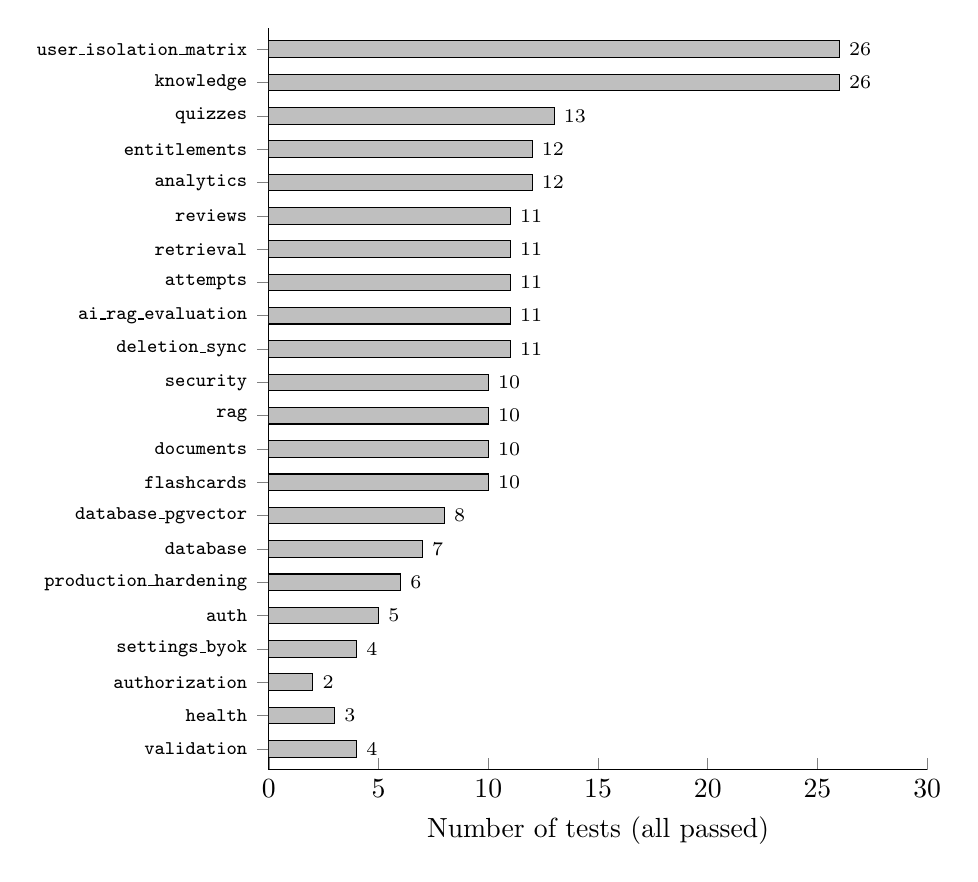
\begin{tikzpicture}
\begin{axis}[
  xbar, width=0.82\textwidth, height=11cm,
  bar width=6pt, xmin=0, xmax=30,
  xlabel={Number of tests (all passed)},
  symbolic y coords={validation,health,authorization,settings\_byok,auth,production\_hardening,database,database\_pgvector,flashcards,documents,rag,security,deletion\_sync,ai\_rag\_evaluation,attempts,retrieval,reviews,analytics,entitlements,quizzes,knowledge,user\_isolation\_matrix},
  ytick=data, y tick label style={font=\scriptsize\ttfamily},
  nodes near coords, nodes near coords style={font=\scriptsize},
  enlarge y limits=0.03, axis lines*=left]
\addplot[fill=black!25, draw=black] coordinates {(4,validation) (3,health) (2,authorization) (4,settings\_byok) (5,auth) (6,production\_hardening) (7,database) (8,database\_pgvector) (10,flashcards) (10,documents) (10,rag) (10,security) (11,deletion\_sync) (11,ai\_rag\_evaluation) (11,attempts) (11,retrieval) (11,reviews) (12,analytics) (12,entitlements) (13,quizzes) (26,knowledge) (26,user\_isolation\_matrix)};
\end{axis}
\end{tikzpicture}
\caption{Automated tests per file in \texttt{app/tests} (223 tests, all passed locally)}\label{fig:testchart}
\end{figure}

\paragraph{Coverage.} Statement coverage was measured with \texttt{coverage.py}. Over the application code
(test files excluded) 7{,}142 of 14{,}131 statements were executed, i.e.\ \textbf{50.5\%}. \Cref{tab:coverage}
shows the coverage by area.

\begin{table}[!htbp]
\centering
\caption{Statement coverage by area (\texttt{app/tests} run)}\label{tab:coverage}
\small
\begin{tabularx}{\textwidth}{@{}X r r r@{}}
\toprule
\textbf{Area} & \textbf{Statements} & \textbf{Covered} & \textbf{Coverage}\\
\midrule
\texttt{app/schemas} (request/response models) & 793 & 775 & 98\%\\
\texttt{app/core} (config, security, database, migrations) & 408 & 339 & 83\%\\
\texttt{app/api} (v1 routers) & 1{,}008 & 818 & 81\%\\
\texttt{app/models} (repositories) & 2{,}508 & 1{,}879 & 75\%\\
\texttt{app/services} (domain services) & 3{,}107 & 2{,}193 & 71\%\\
\texttt{app/sync\_service.py} & 436 & 213 & 49\%\\
\texttt{app/database.py} (study database) & 719 & 215 & 30\%\\
\texttt{app/main.py} (study routes) & 2{,}120 & 400 & 19\%\\
\texttt{app/llm\_providers} & 630 & 102 & 16\%\\
\texttt{app/extractors} & 218 & 31 & 14\%\\
\texttt{app/socratic\_drill.py} & 213 & 0 & 0\%\\
\midrule
\textbf{All application code} & \textbf{14{,}131} & \textbf{7{,}142} & \textbf{50.5\%}\\
\bottomrule
\end{tabularx}
\end{table}

\section{System Testing (UAT, PT, VT)}\label{sec:uat}

\paragraph{User acceptance testing (UAT).} Md.\ Rony Hossain organised informal user-testing sessions during
development with six students, including one team member, referred to here as P1--P6: five study Computer Science
and Engineering and one studies Mechanical Engineering. The participants used the application and gave feedback on
five areas: authentication, the user interface and user experience, reading PDFs, Socratic grading, and flashcards.
The sessions were informal, and \textbf{no metrics were recorded}: there are no task times, completion rates or
questionnaire scores to report. The feedback took the form of five feature requests, listed in \Cref{tab:uat} with
their status in the current build, checked against the code at commit \texttt{60d40f9}.

\begin{table}[!htbp]
\centering
\caption{Feature requests from the user-testing sessions and their status in the current build}\label{tab:uat}
\small\setlength{\tabcolsep}{4pt}
\begin{tabularx}{\textwidth}{@{}l >{\raggedright\arraybackslash}p{0.27\textwidth} l X@{}}
\toprule
\textbf{\#} & \textbf{Request} & \textbf{Status} & \textbf{Evidence in the code}\\
\midrule
1 & Open the PDF view by default when a document is opened & Addressed & The book view starts in PDF mode
(\texttt{viewMode} defaults to \texttt{'pdf'} in \texttt{BookDetailView.tsx}, changed in commit \texttt{eb6f735},
5~Nov~2026)\\
2 & Let the user choose the number of flashcards instead of a fixed 3 or 5 & Addressed & The flashcard-set dialog has a
slider from 1 to 50 (API field \texttt{count}, 1--50, default 10); the topic generator has a slider from 1 to 10, the
PDF command palette accepts 1--20, and the side widget offers 3, 5, 8 or 10\\
3 & Add an OpenRouter provider option & Addressed & An OpenRouter provider is implemented in
\texttt{llm\_providers/factory.py} and the v1 AI service, Settings shows an OpenRouter card, and the provider runs
with a server key in \texttt{.env}. Saving a personal OpenRouter key in the encrypted vault is a planned future
enhancement\\
4 & View and read handwritten PDFs like text PDFs & Addressed & Handwritten pages are read with the Marker
extractor, installed locally or used through the Datalab API with a Datalab key, and the book view offers a
handwriting re-parse. Built-in OCR without Marker is a planned future enhancement\\
5 & Add AI note-creation support & Addressed & Cornell notes are generated per topic
(\texttt{POST /topics/\{id\}/notes/scaffold-stream}; TC-MAN-02)\\
\bottomrule
\end{tabularx}
\end{table}

\paragraph{Performance testing (PT).} RecaLL serves one user on one machine, so performance was measured as
the latency of single requests and the memory of the backend rather than as throughput. The measurements were
made on 18 November 2026 on Md.\ Rony Hossain's laptop (AMD Ryzen~7, 16~GB RAM, Windows~11) with the team's
own uploaded documents, Gemini \texttt{gemini-3.6-flash}, and the backend running in-process.
\Cref{tab:perf} gives the results. The AI timings include waiting at the Gemini free-tier limit of 5 requests
per minute, which the application enforces.

\begin{table}[!htbp]
\centering
\caption{Measured performance with the team's documents (18 November 2026)}\label{tab:perf}
\small
\begin{tabularx}{\textwidth}{@{}X l l@{}}
\toprule
\textbf{Measurement} & \textbf{Runs} & \textbf{Result}\\
\midrule
Backend memory (resident set) & -- & 119~MB idle; 381~MB peak during AI work\\
Backend start-up & 1 & 2.5~s\\
Process a topic (text and AI concepts), CUET AI lecture & 3 & 7.3, 18.4, 50.5~s (median 18.4~s)\\
Generate a Cornell note & 3 & 26.2, 27.9, 47.9~s (median 27.9~s)\\
Generate a Socratic drill (2 questions) & 3 & 42.7, 52.9, 66.0~s (median 52.9~s)\\
Grade a drill answer & 4 & 3.3--35.8~s\\
Knowledge Hub answer (complete) & 6 & 4.9--44.8~s (median 15.9~s)\\
Explain a highlighted passage & 1 & completed and saved (TC-MAN-07)\\
\bottomrule
\end{tabularx}
\end{table}

\paragraph{Volume testing (VT).} The largest document in the team's library is the Pressman textbook
\emph{Software Engineering: A Practitioner's Approach} (7th edition): 930 pages and 20~MB. Its full text
(2.5~million characters) was extracted with PyMuPDF in 3.1~s; it is stored as 933 chunks, and a hybrid search
restricted to it returned in 0.72~s. The whole library holds 11 documents, 1{,}070 chunks and 1{,}326 topics in
a 20.8~MB application database, and the reader and search stayed responsive.

\section{Security Testing (VAPT)}\label{sec:vapt}

Security testing combined the automated security tests above (authentication, isolation, cryptography,
injection) with a manual review of the routes and of the key-handling code. The backend binds only to
\texttt{127.0.0.1}, so it cannot be reached from another computer. \Cref{tab:vapt} lists the protections that
were verified, each by passing tests in \texttt{app/tests}.

\begin{table}[!htbp]
\centering
\caption{Verified security protections}\label{tab:vapt}
\small
\begin{tabularx}{\textwidth}{@{}>{\raggedright\arraybackslash}p{0.30\textwidth} X l@{}}
\toprule
\textbf{Protection} & \textbf{Evidence (tests)} & \textbf{Status}\\
\midrule
Cross-user isolation of documents, conversations, cards, quizzes, reviews and keys & 26 tests in \texttt{test\_user\_isolation\_matrix} & Verified\\
Tampered JWT rejected & \texttt{test\_jwt\_tampered\_token\_rejected}, \texttt{test\_jwt\_token\_expiration} & Verified\\
Tampered ciphertext rejected (AES-GCM tag check) & \texttt{test\_aes\_256\_gcm\_tamper\_detection} & Verified\\
Prompt-injection delimiters sanitised & \texttt{test\_prompt\_injection\_delimiter\_sanitization}, \texttt{test\_prompt\_injection\_defense} & Verified\\
Password hashing with a unique salt (PBKDF2-HMAC-SHA256) & \texttt{test\_password\_hashing\_and\_verification}, \texttt{test\_password\_salt\_uniqueness} & Verified\\
Rate limiting of authentication requests and uploads & \texttt{test\_password\_change\_rate\_limiting}, \texttt{test\_upload\_rate\_limiting} & Verified\\
Production start-up refuses default secrets & \texttt{test\_production\_secret\_rejection}, \texttt{test\_production\_settings\_reject\_default\_dev\_secrets} & Verified\\
\bottomrule
\end{tabularx}
\end{table}

\section{AI-specific Testing}

\begin{itemize}
  \item \textbf{Grounding and hallucination.} Eleven tests in \texttt{test\_ai\_rag\_evaluation.py} check direct,
  semantic and multi-chunk retrieval, the ``not in the material'' answer, tenant isolation and document scope, and
  that citations to chunks that were not retrieved are removed. The same checks were also made manually with
  documents the team had uploaded (TC-MAN-05).
  \item \textbf{Robustness of parsing.} Replies wrapped in Markdown fences or with broken JSON are repaired and
  validated (TC-GEN-08); invalid quiz options are rejected (TC-GEN-06).
  \item \textbf{Prompt injection.} Document text that tries to close the \texttt{<reference\_data>} tag is
  neutralised (TC-KH-06).
  \item \textbf{Model quality with a real provider.} Because CI runs without keys, live quality was checked with
  Gemini \texttt{gemini-3.6-flash} on the team's documents. All 7 structured replies (3 drill generations and
  4 gradings) were valid, and every drill had exactly two questions of the required types. Grading followed the
  score bands: answers built from the key ideas scored 95 and 100 (mastered, no cards), and an
  ``I am not sure'' answer scored 0 (misconception, 2 cards each time). In the Knowledge Hub, all 5 answerable
  questions cited the relevant pages, for example the Turing Test on page 25 and Claude Shannon on page 43 of the
  AI lecture, and a question about a topic not in the selected document was answered as not covered by the
  materials.
\end{itemize}

\section{Assessment of the Goodness of the Test Suite}\label{sec:goodness}

\paragraph{Strengths.} The suite is large (223 automated tests) and deterministic: it runs without network access
or keys, and all 223 tests pass. It is strongest where failures would be most harmful: user
isolation (26 tests), authentication, key encryption and FSRS scheduling. Statement coverage of the
\texttt{/api/v1} routers, schemas, core and services is between 71\% and 98\%.

\paragraph{Future improvements.}
\begin{itemize}
  \item Extend the automated tests to the study features (reader, Cornell notes and Socratic drill), which are
  tested manually today, to raise the overall statement coverage of 50.5\%.
  \item Add branch coverage and mutation testing.
  \item Run the nine Playwright end-to-end journeys as part of every test run.
\end{itemize}

\paragraph{Effectiveness.} The automated suite and the manual tests together cover every requirement in
\Cref{tab:trace}. Defects found during development and user testing were fixed by Turjo and Saimun.
